% Chapter Template

\chapter{Ensayos y Resultados} % Main chapter title

\label{Chapter4} % Change X to a consecutive number; for referencing this chapter elsewhere, use \ref{ChapterX}

En este capítulo se detallan los ensayos realizados para comprobar el correcto funcionamiento del firmware de los nodos y el {\textit{Gateway}}, como así también del sistema en general.
%----------------------------------------------------------------------------------------
%	SECTION 1
%----------------------------------------------------------------------------------------

\section{Ensayos de comunicación}
\label{sec:pruebasHW}

En esta sección se detallan los ensayos de comunicación entre el nodo y el {\textit{gateway}} a partir de una terminal de comandos en Linux. Estos ensayos son muy importantes debido a que la comunicación inalámbrica es el requerimiento principal del proyecto. El objetivo es comprobar que existe una correcta comunicación entre los dos dispositivos.

\subsection{Banco de pruebas}

El banco de pruebas de ésta sección se componen de los elementos listados en la tabla [\ref{tab:bancodepruebas1}] :

\begin{table}[h]
	\centering
	\caption[Banco de pruebas 1]{Banco de pruebas para ensayos de comunicación}
	\begin{tabular}{l c m{7.5cm}}    
		\toprule
		\textbf{Componentes}  		& \textbf{Pertenencia}     	& \textbf{Función}																				\\
		\midrule
		Raspberry Pi				& \ Gateway 				& \ Funciona como nexo entre entre el transceptor y una terminal para enviar comandos por UART.	\\
		Transceptor LoRa 			& \ Gateway					& \ Conectado a través de la UART, recibe comandos y los envía por LoRa (915 MHz). 				\\
		Display	 					& \ Gateway 				& \ Conectado al puerto HDMI de la raspberry pi. 												\\
		Transceptor LoRa		 	& \ Nodo 					& \ Recibe comandos por LoRa, los procesa, ejecuta y envía una respuesta.						\\
		\bottomrule
		\hline
	\end{tabular}
	\label{tab:bancodepruebas1}
\end{table}

La propuesta de éste banco es la de tener los componentes mínimos y necesarios al hacer las pruebas de conectividad y de {\textit{Set/Get}} mediante una terminal de comandos. En la figura [\ref{fig:bancodepruebas1}] se puede ver el esquema de conexión básico.

\begin{figure}[ht!]
	\centering
	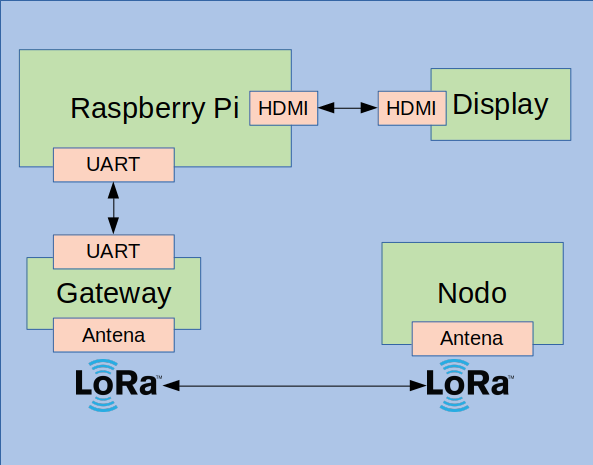
\includegraphics[width=0.5\textwidth]{./Figures/bancodepruebas.png}
	\caption{Banco de pruebas para el ensayo de comunicación.}
	\label{fig:bancodepruebas1}
\end{figure}

\subsection{Pruebas}

\subsubsection{Pruebas de conexión}
El nodo posee dos estados de conectividad inalámbrica, éstos estados son conectado y desconectado. En ésta prueba se logra realizar la conexión inalámbrica de un nodo con el {\textit{gateway}}. Los pasos realizados fueron los siguientes:

\begin{enumerate}
\item Con el nodo encendido, presionar el botón {\textit{Modo}} por seis segundos.
\end{enumerate}

En la figura [\ref{fig:conexion}] se puede ver que el {\textit{gateway}} recibe el comando NODE:ID, donde ID corresponde al nodo utilizado. Cuando el {\textit{gateway}} recibe éste comando, envía un {\textit{ACK}} al nodo y éste pasa al estado conectado.

\begin{figure}[h!]
	\centering
	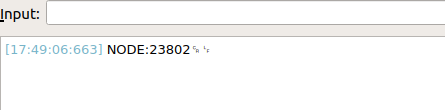
\includegraphics[width=0.5\textwidth]{./Figures/conexion.png}
	\caption{Ensayo de conexión de un nuevo nodo.}
	\label{fig:conexion}
\end{figure}

\subsubsection{Pruebas de Set y Get}
Las pruebas realizadas en esta sección corresponden al envío de comandos para configurar o setear algún parámetro del nodo y también recibir información de éste.
Los pasos realizados fueron los siguientes:

\begin{enumerate}
\item Enviar el comando {\textit{Get}} y esperar a recibir un array de datos.
\item Enviar el comando correspondiente para configurar el estado del sistema al modo {\textit{Manual}} y esperar un {\textit{ACK}}.
\item Enviar nuevamente el comando {\textit{Get}} para corroborar el seteo del parámetro.
\end{enumerate}

En la figura [\ref{fig:image1}] se puede ver el paso 1, donde en la figura [\ref{fig:get1}] se envía el comando y en la figura [\ref{fig:get2}] se recibe el {\textit{ACK}}.

\begin{figure}[h]

\begin{subfigure}{0.5\textwidth}
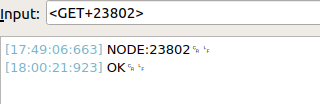
\includegraphics[width=1\textwidth]{./Figures/GET1.png}
\caption{Envío del comando {\textit{Get}} por consola al puerto serie.}
\label{fig:get1}
\end{subfigure}
\begin{subfigure}{0.5\textwidth}
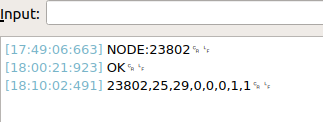
\includegraphics[width=1\textwidth]{./Figures/GET2.png}
\caption{Recepción de datos enviados por el nodo.}
\label{fig:get2}
\end{subfigure}

\caption{}
\label{fig:image1}
\end{figure}

En la figura [\ref{fig:image2}] se puede ver el paso 2, donde en la figura [\ref{fig:confmanual1}] se envía el comando y en la [\ref{fig:confmanual2}] se recibe el {\textit{ACK}}.

\begin{figure}[h]

\begin{subfigure}{0.5\textwidth}
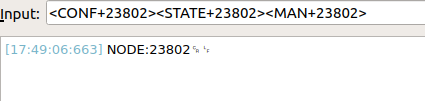
\includegraphics[width=1\textwidth]{./Figures/CONFMANUAL1.png}
\caption{Envío del comando {\textit{Conf}} para poner el sistema en modo manual.}
\label{fig:confmanual1}
\end{subfigure}
\begin{subfigure}{0.5\textwidth}
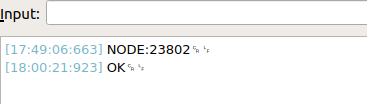
\includegraphics[width=1\textwidth]{./Figures/CONFMANUAL2.png}
\caption{Recepción del comando {\textit{Ok}} enviado por el nodo.}
\label{fig:confmanual2}
\end{subfigure}

\caption{}
\label{fig:image2}
\end{figure}

Finalmente en la figura [\ref{fig:confmanual3}] se puede ver la recepción del comando {\textit{Get}} que corresponde al paso 3 y se corrobora el cambio en el parámetro.

\begin{figure}[ht!]
	\centering
	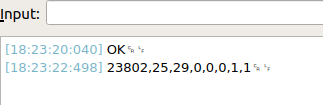
\includegraphics[width=0.5\textwidth]{./Figures/CONFMANUAL3.png}
	\caption{Recepción de datos enviados por el nodo.}
	\label{fig:confmanual3}
\end{figure}


\subsubsection{Resultados}

\begin{itemize}
\item Se comprobó que la arquitectura de comandos utilizada funciona correctamente.
\item El envío y recepción de datos toma un tiempo menor a 2 segundos por comando.
\item El nodo procesa satisfactoriamente la información.
\end{itemize}


\section{Ensayos de sensores y actuadores}

En esta sección se detallan los ensayos de uso de los periféricos en el nodo, comandados por el {\textit{gateway}}. El objetivo de estos ensayos es corroborar el correcto funcionamiento de la placa de circuitos impreso desarrollada, como también los sensores y actuadores utilizados.

\subsection{Banco de pruebas}

El banco de pruebas de ésta sección se componen de los elementos listados en la tabla [\ref{tab:bancodepruebas2}]:

\begin{table}[h]
	\centering
	\caption[Banco de pruebas 2]{Banco de pruebas para ensayos de comunicación}
	\begin{tabular}{l c m{7.5cm}}    
		\toprule
		\textbf{Componentes}  		& \textbf{Pertenencia}     	& \textbf{Función}																				\\
		\midrule
		Raspberry Pi				& \ Gateway 				& \ Funciona como nexo entre entre el transceptor y una terminal para enviar comandos por UART.	\\
		Transceptor LoRa 			& \ Gateway					& \ Conectado a través de la UART, recibe comandos y los envía por LoRa (915 MHz). 				\\
		Display	 					& \ Gateway 				& \ Conectado al puerto HDMI de la raspberry pi. 												\\
		Transceptor LoRa		 	& \ Nodo 					& \ Recibe comandos por LoRa, los procesa, ejecuta y envía una respuesta.						\\
		Periféricos		 			& \ Nodo 					& \ Sensor de movimiento, sensor de temperatura y humedad, relay y led infrarrojo				\\
		\bottomrule
		\hline
	\end{tabular}
	\label{tab:bancodepruebas2}
\end{table}

En la figura [\ref{fig:bancodepruebas2}] se puede ver el esquema de conexionado básico.

\begin{figure}[h!]
	\centering
	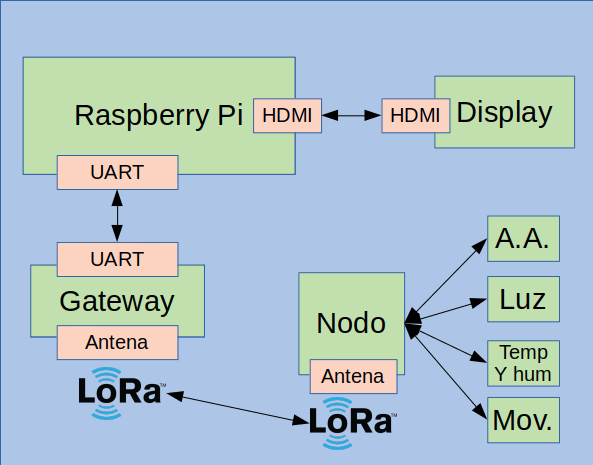
\includegraphics[width=0.5\textwidth]{./Figures/bancodepruebas1.png}
	\caption{Banco de pruebas para el ensayo de sensores y actuadores.}
	\label{fig:bancodepruebas2}
\end{figure}

\subsection{Pruebas}

Las pruebas realizadas fueron de encendido y apagado de luz y aire acondicionado, detección de movimiento y sensado de temperatura y humedad.

Se comprobó el correcto funcionamiento de forma visual en los dispositivos y además utilizando el comando {\textit{Get}} para determinar si hubo un cambio en el estado de las salidas.

\subsubsection{Pruebas de encendido y apagado de luces}

Los pasos realizados en éste ensayo fueron los siguientes:

\begin{enumerate}
\item Enviar el comando para encender la luz, esperar un {\textit{ACK}}.
\item Enviar el comando {\textit{Get}} y esperar un array de datos de respuesta.
\item Enviar el comando para apagar la luz, esperar un {\textit{ACK}}.
\item Enviar el comando {\textit{Get}} y esperar un array de datos de respuesta.
\end{enumerate}

En la figura [\ref{fig:image3}] se puede ver el paso 1 y 2, donde en la figura [\ref{fig:luz1}] se envía el comando y en la figura [\ref{fig:luz2}] se recibe el {\textit{ACK}} y el array de datos.

\begin{figure}[h]

\begin{subfigure}{0.5\textwidth}
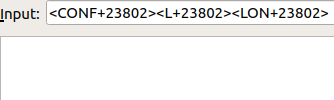
\includegraphics[width=1\textwidth]{./Figures/luz1.png}
\caption{Envío de comando para encender la luz.}
\label{fig:luz1}
\end{subfigure}
\begin{subfigure}{0.5\textwidth}
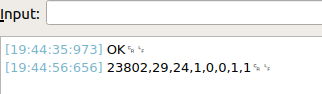
\includegraphics[width=1\textwidth]{./Figures/luz2.png}
\caption{Recepción de datos.}
\label{fig:luz2}
\end{subfigure}

\caption{}
\label{fig:image3}
\end{figure}

En la figura [\ref{fig:image4}] se puede ver el paso 3 y 4, donde en la figura [\ref{fig:luz3}] se envía el comando y en la figura [\ref{fig:luz4}] se recibe el {\textit{ACK}} y el array de datos.

\begin{figure}[h]

\begin{subfigure}{0.5\textwidth}
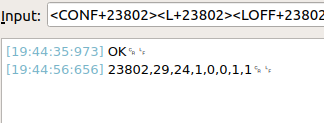
\includegraphics[width=1\textwidth]{./Figures/luz3.png}
\caption{Envío de comando para apagar la luz.}
\label{fig:luz3}
\end{subfigure}
\begin{subfigure}{0.5\textwidth}
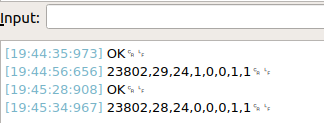
\includegraphics[width=1\textwidth]{./Figures/luz4.png}
\caption{Recepción de datos.}
\label{fig:luz4}
\end{subfigure}

\caption{}
\label{fig:image4}
\end{figure}

Si se comparan los dos arrays de datos en la figura [\ref{fig:luz4}] se puede ver claramente el cambio de la variable en la columna 4.

\subsubsection{Pruebas de encendido y apagado de aire acondicionado}

Los pasos realizados en éste ensayo fueron los siguientes:

\begin{enumerate}
\item Enviar cambio de protocolo de aire acondicionado y esperar un {\textit{ACK}}.
\item Enviar el comando para encender el aire acondicionado, esperar un {\textit{ACK}}.
\item Enviar el comando {\textit{Get}} y esperar un array de datos de respuesta.
\item Enviar el comando para apagar el aire acondicionado, esperar un {\textit{ACK}}.
\item Enviar el comando {\textit{Get}} y esperar un array de datos de respuesta.
\end{enumerate}

En la figura [\ref{fig:aa1}] se puede ver la secuencia de comandos recibidos por el {\textit{gateway}} correspondiente a la secuencia descrita anteriormente.

\begin{figure}[h!]
	\centering
	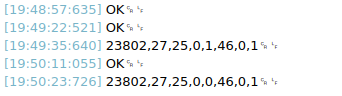
\includegraphics[width=0.55\textwidth]{./Figures/aa1.png}
	\caption{Respuestas del nodo a los comandos utilizados.}
	\label{fig:aa1}
\end{figure}

Si se comparan los dos arrays de datos en la figura [\ref{fig:aa1}] se puede ver claramente el cambio de la variable en la columna 5.

\subsubsection{Pruebas de sensores}

El sistema posee dos sensores, un sensor de humedad y temperatura y un sensor de movimiento. El objetivo de este ensayo es corroborar el correcto funcionamiento de estos. Los pasos para los ensayos del sensor de temperatura y humedad fueron los siguientes:

\begin{enumerate}
\item Enviar el comando {\textit{Get}} para conocer el valor de temperatura y humedad actual.
\item Acercar una fuente de calor al sensor.
\item Enviar el comando {\textit{Get}} para corroborar el cambio de temperatura y humedad.
\end{enumerate}

En la figura [\ref{fig:sensores1}] se puede ver la respuesta del sensor a los dos envíos del comando {\textit{Get}} y se puede corroborar que los valores de temperatura y humedad han cambiado. Estos valor se pueden ver en el array, en las columnas 2 (temperatura) y 3(humedad).

\begin{figure}[h!]
	\centering
	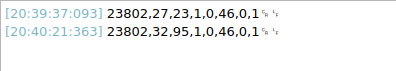
\includegraphics[width=0.55\textwidth]{./Figures/sensores1.png}
	\caption{Respuesta al cambio de temperatura y humedad en el nodo.}
	\label{fig:sensores1}
\end{figure}

Finalmente se hizo el ensayo del sensor de movimiento, para el que se siguieron los pasos:

\begin{enumerate}
\item Enviar el comando para cambiar el estado del sistema a {\textit{Automático}} y esperar un {\textit{ACK}}.
\item Enviar el comando para activar el sensor de movimiento y esperar un {\textit{ACK}}.
\item Mover un objeto frente al sensor de movimiento.
\end{enumerate}

En la figura [\ref{fig:sensores2}] se puede ver la secuencia descrita anteriormente. Se reciben los dos {\textit{ACK}} y luego se procede al paso 3 que genera el envío del comando de alarma del nodo al {\textit{gateway}}.

\begin{figure}[h!]
	\centering
	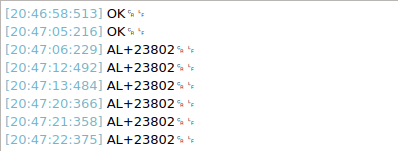
\includegraphics[width=0.55\textwidth]{./Figures/sensores2.png}
	\caption{Pruebas del sensor de movimiento.}
	\label{fig:sensores2}
\end{figure}

\subsubsection{Resultados}

\begin{itemize}
\item Se comprobó que los sensores y actuadores funcionan correctamente.
\item El envío de datos al sensar movimiento tiene un tiempo menor a 2 segundos y lo hace de forma correcta.
\item El circuito impreso desarrollado funciona correctamente.
\end{itemize}


\section{Ensayos de integración}

En esta sección se detallan los ensayos de comunicación entre el nodo y el {\textit{gateway}}, para ello se utiliza una interfaz web y un proceso programado en {\textit{Python}} que maneja las peticiones de la interfaz de usuario creada en {\textit{Node-red}}. El objetivo de estos ensayos es corroborar el correcto funcionamiento del sistema con el agregado de la interfaz web y simulando el sistema completo.

\subsection{Banco de pruebas}

El banco de pruebas de ésta sección se componen de los elementos listados en la tabla [\ref{tab:bancodepruebas3}]:

\begin{table}[h]
	\centering
	\caption[Banco de pruebas 3]{Banco de pruebas para ensayos de comunicación}
	\begin{tabular}{l c m{7.5cm}}    
		\toprule
		\textbf{Componentes}  		& \textbf{Pertenencia}     	& \textbf{Función}																				\\
		\midrule
		Raspberry Pi				& \ Gateway 				& \ Ejecuta la aplicación programada en {\textit{Python}} y la interfaz web.	\\
		Transceptor LoRa 			& \ Gateway					& \ Conectado a través de la UART, recibe comandos y los envía por LoRa (915 MHz). 				\\
		Display	 					& \ Gateway 				& \ Conectado al puerto HDMI de la raspberry pi. 												\\
		Transceptor LoRa		 	& \ Nodo 					& \ Recibe comandos por LoRa, los procesa, ejecuta y envía una respuesta.						\\
		Periféricos		 			& \ Nodo 					& \ Sensor de movimiento, sensor de temperatura y humedad, relay y led infrarrojo				\\
		\bottomrule
		\hline
	\end{tabular}
	\label{tab:bancodepruebas3}
\end{table}

En la figura [\ref{fig:bancodepruebas3}] se puede ver el esquemático básico del sistema. Se utiliza la ventana de comandos con el motivo de mostrar que los comandos son enviados correctamente cuando se interactúa con la interfaz web. 

\begin{figure}[ht!]
	\centering
	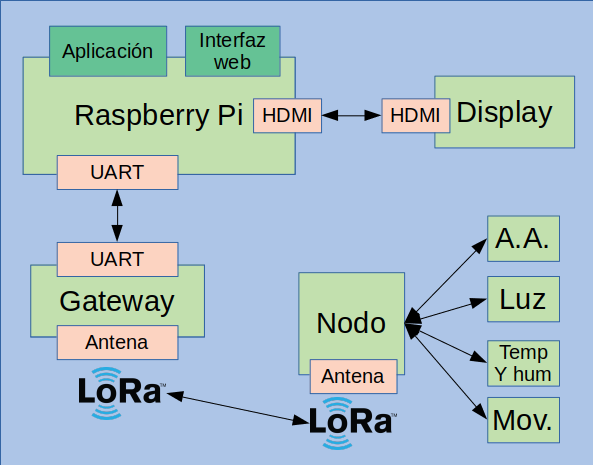
\includegraphics[width=0.5\textwidth]{./Figures/bancodepruebas2.png}
	\caption{Banco de prueba para ensayos de integración.}
	\label{fig:bancodepruebas3}
\end{figure}


\subsection{Pruebas}

Las pruebas realizadas se detallan en la siguiente lista:

\begin{enumerate}
\item Ensayo de conexión con interfaz y aplicación.
\item Ensayo de encendido y apagado de luz.
\item Ensayo de encendido y apagado de aire acondicionado.
\item Ensayo de sensor de temperatura y humedad.
\item Ensayo de sensor de movimiento.
\end{enumerate}

\subsubsection{Pruebas de conexión con interfaz y aplicación}

Se realizó el ensayo de conexión de un nodo al sistema mediante el uso de la interfaz web. Para ello se siguen los pasos:

\begin{enumerate}
\item Hacer click en la solapa {\textit{Configuración}}.
\item Hacer click en {\textit{Agregar nuevo dispositivo}}.
\item Presionar el botón {\textit{Modo}} del nodo durante seis segundos.
\end{enumerate}

En las figuras [\ref{fig:interfaz1}] y [\ref{fig:interfaz2}] se ven los pasos 1 y 2. Aquí se selecciona la solapa de configuración para tener disponible el botón de agregado de un nodo al sistema.

\begin{figure}[ht!]
	\centering
	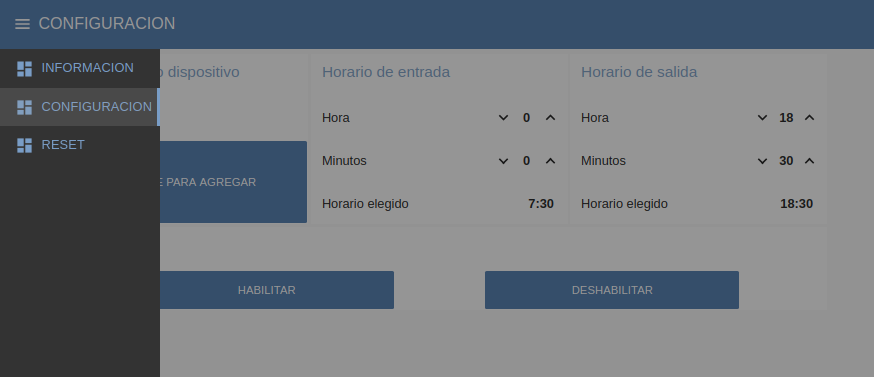
\includegraphics[width=0.8\textwidth]{./Figures/interfaz1.png}
	\caption{Solapa de configuración.}
	\label{fig:interfaz1}
\end{figure}

\begin{figure}[ht!]
	\centering
	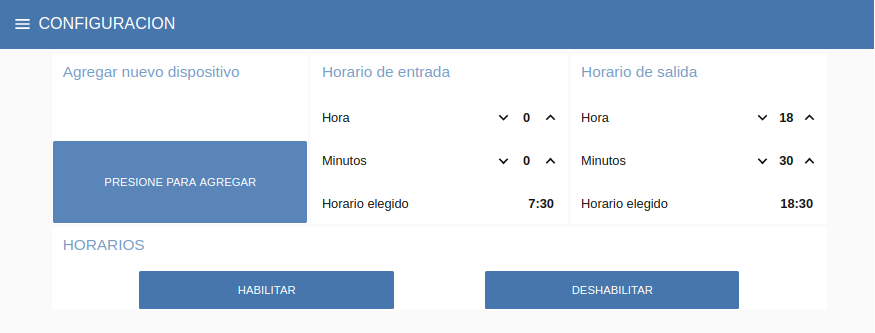
\includegraphics[width=0.8\textwidth]{./Figures/interfaz2.png}
	\caption{Ventana de configuración.}
	\label{fig:interfaz2}
\end{figure}

En la figura [\ref{fig:interfaz3}] se muestra la terminal de Linux en la que luego del paso 3 mencionado, llega el comando NODE:ID correspondiente al nodo en cuestión. Finalmente el sistema escribe en un archivo de log, la línea que se muestra en la parte inferior de la figura.

\begin{figure}[ht!]
	\centering
	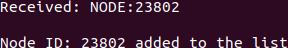
\includegraphics[width=0.5\textwidth]{./Figures/interfaz3.png}
	\caption{Terminal de comandos muestra recepción del nodo.}
	\label{fig:interfaz3}
\end{figure}

\subsubsection{Pruebas de encendido y apagado de luz}

Se realizó el ensayo de encendido y apagado de luz mediante el uso de los botones ON y OFF de la interfaz web, correspondientes al nodo en cuestión. Para ello se siguen los pasos:

\begin{enumerate}
\item Hacer click en la solapa {\textit{Información}}.
\item Hacer click en {\textit{ON}}.
\item Hacer click en {\textit{OFF}}.
\end{enumerate}

En la figura [\ref{fig:interfaz4}] se puede ver el paso 1, aquí se selecciona la solapa de información que se encuentra en la parte izquierda de la pagina web.

\begin{figure}[ht!]
	\centering
	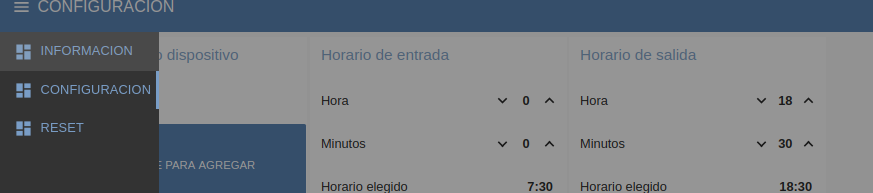
\includegraphics[width=0.8\textwidth]{./Figures/interfaz4.png}
	\caption{Solapa de información.}
	\label{fig:interfaz4}
\end{figure}

En la figura [\ref{fig:interfaz52}] se muestran los botones que provee la pagina web para el encedido y apagado de luz, también se ve el estado actual. Una vez presionado el botón {\textit{ON}} se puede ver en la figura [\ref{fig:interfaz51}] el envío del comando al nodo y la recepción del {\textit{ACK}}. Luego el sistema envía el comando {\textit{Get}} automáticamente para corroborar el cambio y actualizar el estado en la interfaz web.

\begin{figure}[h!]
	\centering
	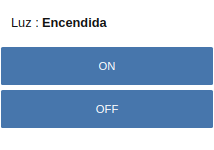
\includegraphics[width=0.3\textwidth]{./Figures/interfaz52.png}
	\caption{Interfaz web luego de presionar el botón {\textit{ON}}.}
	\label{fig:interfaz52}
\end{figure}

\begin{figure}[h!]
	\centering
	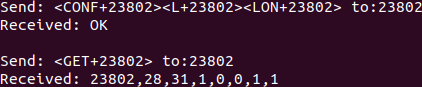
\includegraphics[width=0.6\textwidth]{./Figures/interfaz51.png}
	\caption{Envío y recepción de comandos después de presionar el botón {\textit{ON}}.}
	\label{fig:interfaz51}
\end{figure}

En las figuras [\ref{fig:interfaz62}] y [\ref{fig:interfaz61}] se puede ver el mismo mecanismo utilizado anteriormente en las figuras [\ref{fig:interfaz52}] y [\ref{fig:interfaz51}] pero en este caso se apaga la luz.

\begin{figure}[h!]
	\centering
	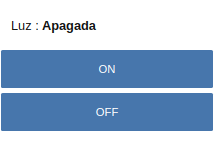
\includegraphics[width=0.3\textwidth]{./Figures/interfaz62.png}
	\caption{Interfaz web luego de presionar el botón {\textit{OFF}}.}
	\label{fig:interfaz62}
\end{figure}

\begin{figure}[h!]
	\centering
	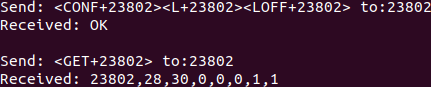
\includegraphics[width=0.6\textwidth]{./Figures/interfaz61.png}
	\caption{Envío y recepción de comandos después de presionar el botón {\textit{OFF}}.}
	\label{fig:interfaz61}
\end{figure}


\subsubsection{Pruebas de encendido y apagado del aire acondicionado}

De la misma manera que en la prueba anterior,se procedió a ensayar el encendido y apagado del aire acondicionado, para ésto se siguen los pasos:

\begin{enumerate}
\item Hacer click en la solapa {\textit{Información}}.
\item Elegir la marca del aire acondicionado.
\item Hacer click en {\textit{ON}}.
\item Hacer click en {\textit{OFF}}.
\end{enumerate}

En la figura [\ref{fig:interfaz71}] se muestra la apertura del menú que contiene las marcas de aires acondicionados y se selecciona una.
%
\begin{figure}[h!]
	\centering
	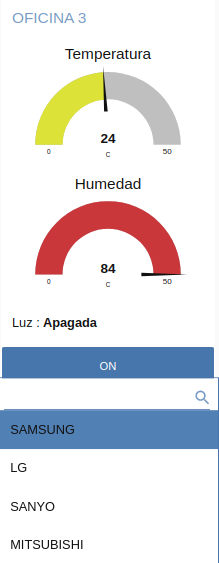
\includegraphics[width=0.2\textwidth]{./Figures/interfaz71.png}
	\caption{Selección de la marca del aire acondicionado en la interfaz de usuario.}
	\label{fig:interfaz71}
\end{figure}

Una vez seleccionada la marca, se muestra en la figura [\ref{fig:interfaz70}] el correspondiente envío del comando al nodo y la respuesta de éste.

\begin{figure}[h!]
	\centering
	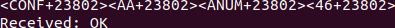
\includegraphics[width=0.6\textwidth]{./Figures/interfaz70.png}
	\caption{Envío y recepción de comandos por la terminal.}
	\label{fig:interfaz70}
\end{figure}

En la figura [\ref{fig:interfaz72}] se muestra el estado actual y los botones que provee la interfaz para el encendido y apagado del aire acondicionado.

\begin{figure}[h!]
	\centering
	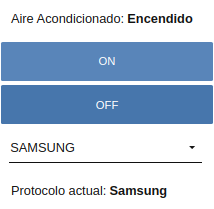
\includegraphics[width=0.3\textwidth]{./Figures/interfaz72.png}
	\caption{Interfaz web luego de presionar el botón {\textit{ON}}.}
	\label{fig:interfaz72}
\end{figure}

En la figura [\ref{fig:interfaz73}] se ve el envío del comando de encendido del aire acondicionado y la respuesta del nodo.

\begin{figure}[h!]
	\centering
	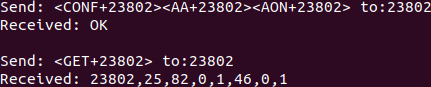
\includegraphics[width=0.6\textwidth]{./Figures/interfaz73.png}
	\caption{Envío y recepción de comandos por la terminal.}
	\label{fig:interfaz73}
\end{figure}

En las figuras [\ref{fig:interfaz81}] y [\ref{fig:interfaz82}] se puede ver el mismo mecanismo utilizado anteriormente en las figuras [\ref{fig:interfaz72}] y [\ref{fig:interfaz73}] pero en este caso se apaga el aire acondicionado.

\begin{figure}[ht!]
	\centering
	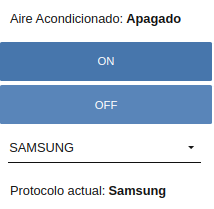
\includegraphics[width=0.3\textwidth]{./Figures/interfaz81.png}
	\caption{Interfaz web luego de presionar el botón {\textit{OFF}}.}
	\label{fig:interfaz81}
\end{figure}

\begin{figure}[ht!]
	\centering
	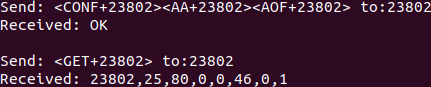
\includegraphics[width=0.6\textwidth]{./Figures/interfaz82.png}
	\caption{Envío y recepción de comandos por la terminal.}
	\label{fig:interfaz82}
\end{figure}


\subsubsection{Pruebas de sensor de temperatura y humedad}

En este ensayo se corrobora que los datos mostrados en la interfaz web acerca del sensor de temperatura y humedad se corresponden con los datos recibidos por el nodo.

En las figura [\ref{fig:interfaz90}] se pueden ver los datos recibidos por el nodo luego de que el sistema le mande un comando {\textit{Get}} al nodo, en las columnas 2 y 3 se puede ver el valor de temperatura y humedad respectivamente, y en la figura [\ref{fig:interfaz91}] se muestra la interfaz web y se corrobora el correcto funcionamiento de la interfaz mostrando los valores reales recibidos.

\begin{figure}[ht!]
	\centering
	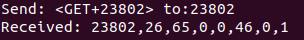
\includegraphics[width=0.5\textwidth]{./Figures/interfaz90.png}
	\caption{Recepción de datos, después del envío del comando {\textit{Get}} }
	\label{fig:interfaz90}
\end{figure}

\begin{figure}[ht!]
	\centering
	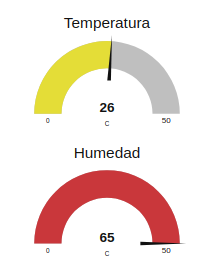
\includegraphics[width=0.3\textwidth]{./Figures/interfaz91.png}
	\caption{Interfaz web con los datos de temperatura y humedad}
	\label{fig:interfaz91}
\end{figure}

\subsubsection{Pruebas de detección de movimiento}

En esta sección se ensaya el uso del sensor de movimiento. Los pasos realizados fueron:

\begin{enumerate}
\item Hacer click en la solapa {\textit{Información}}.
\item Poner el sistema en modo Automático.
\item Activar la detección de movimiento.
\end{enumerate}

El sistema se pone en modo automático mediante el uso del botón {\textit{Modo}} que se encuentra en el nodo, pero también se lo puede hacer mediante la interfaz web.

En la figura [\ref{fig:interfaz10}] se puede ver que la interfaz web nos indica que el sistema se encuentra en modo automático y además provee los botones para activar y desactivar el sensor de movimiento.

\begin{figure}[h!]
	\centering
	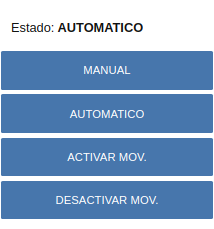
\includegraphics[width=0.3\textwidth]{./Figures/interfaz10.png}
	\caption{Interfaz web con el sistema en modo automático.}
	\label{fig:interfaz10}
\end{figure}

Se puede ver en la figura [\ref{fig:interfaz11}] que luego del paso 3, se activa el sensor de movimiento y al pasar un objeto por delante, el sistema lo detecta y activa una ventana de emergencia en la interfaz web.

\begin{figure}[ht!]
	\centering
	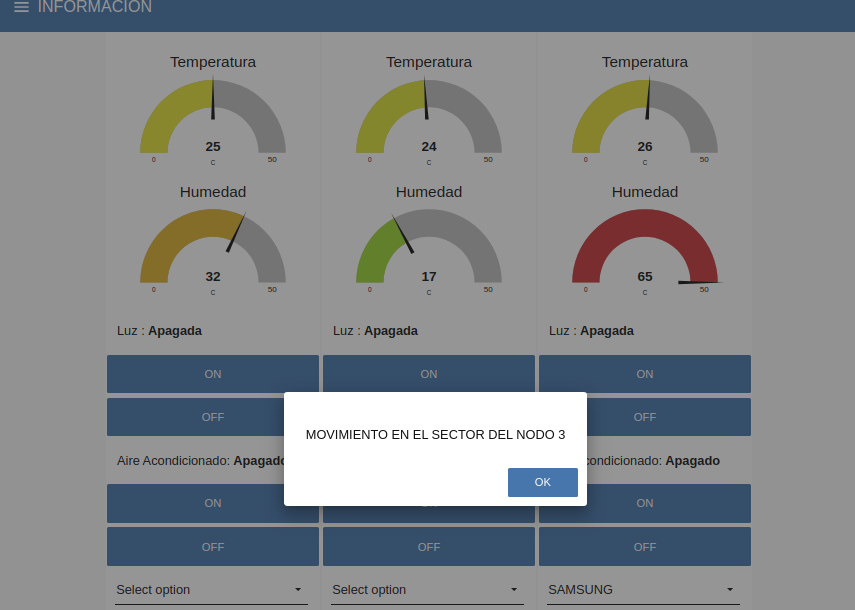
\includegraphics[width=0.8\textwidth]{./Figures/interfaz11.png}
	\caption{Interfaz web con ventana pop-up indicando una alerta de movimiento en el sector 3}
	\label{fig:interfaz11}
\end{figure}


\subsubsection{Resultados}

\begin{itemize}
\item Se comprobó que la interfaz web funciona correctamente.
\item Los comandos son enviados y recibidos correctamente.
\item La sincronización de hilos en la aplicación funciona como es esperado.
\end{itemize}
